\documentclass[11pt,a4paper]{article}
\usepackage[utf8]{inputenc}
\usepackage[T1]{fontenc}
\usepackage{lmodern}
\usepackage[margin=2.5cm]{geometry}
\usepackage{setspace}
\usepackage{booktabs,tabularx}
\usepackage{xcolor}
\usepackage{tikz}
\usetikzlibrary{positioning,arrows.meta}
\usepackage[hidelinks]{hyperref}
\usepackage{parskip}
\onehalfspacing

\begin{document}

\begin{titlepage}
\centering
{\large Technische Hochschule Deggendorf\par}
{\large MDM-M-2 -- Case Study: Intelligent Systems in Production\par}
\vspace{2cm}
{\LARGE\bfseries Case Study Project\par}
\vspace{0.6cm}
{\Large AI-Driven Multi-Objective Optimization of a Medical Injection-Moulding Line:\\ A Simulated Case Study of Gerresheimer Pfreimd\par}
\vspace{0.6cm}
{\LARGE\bfseries Bibliography Report\par}
\vspace{1.5cm}
{\large Submitted by:\par}
\vspace{0.2cm}
Mahesh Koduri (Matriculation No.: 22407285)\par
Kuriakose Vettikattil Raju, Team Lead (Matriculation No.: 22401909)\par
Saurabhkumar Mahant (Matriculation No.: 12501037)\par
\vspace{1cm}
{\large Course:\par}
M.Eng. in Applied AI for Digital Production Management\par
\vspace{1cm}
{\large Under the Supervision of:\par}
Prof. Dr.-Ing. Hamidreza Heidari\par
\vspace{0.5cm}
Repository: \url{https://github.com/MaheshBhushan/Case-Study-Intelligent-Systems}\par
\vfill
{\large Date of Submission: 03.11.2026\par}
\end{titlepage}

\section*{Abstract}
\addcontentsline{toc}{section}{Abstract}
This report reviews the literature behind our case-study project. The project simulates a five-station medical injection-moulding line (drying, clean-room moulding, camera inspection, assembly and clean-room packaging) modelled on the Gerresheimer plant in Pfreimd, Bavaria. It compares fixed dispatching rules with a predictive, multi-objective scheduling strategy. The review starts with the broad context of Industry~4.0 and artificial intelligence in production planning. It then narrows to four technical areas that the project combines: production scheduling with sequence-dependent setups, energy-efficient scheduling, machine breakdowns with dynamic rescheduling, and predictive maintenance with machine learning. The review also covers discrete-event simulation as the evaluation method and multi-objective optimization as the decision method. Finally, it summarises the domain constraints of medical injection moulding, such as clean-room energy load and Good Manufacturing Practice (GMP) line clearance. Most studies optimise one objective or treat energy, changeovers and failures separately. Few studies evaluate all three together on a reproducible, openly documented simulation of a regulated moulding line. Our project addresses this gap. It uses SimPy for simulation, a failure-risk classifier trained on the public AI4I~2020 dataset, and NSGA-II search in Optuna to explore the trade-offs.

\vspace{0.5em}
\textbf{Keywords:} injection moulding; production scheduling; multi-objective optimization; energy efficiency; machine downtime; discrete-event simulation; predictive maintenance

\newpage
\tableofcontents
\newpage
\listoftables
\listoffigures
\newpage

\section{Introduction}
\subsection{Background: Industry 4.0 and intelligent production}
Industry~4.0 describes the integration of cyber-physical systems, networked sensors and data analytics into manufacturing \cite{kagermann2013}. Lee et al.\ \cite{lee2015} propose a five-level architecture for cyber-physical production systems. The architecture moves from data acquisition, through analytics and digital models, to self-configuring decisions. Their key point for our project is that data only creates value when a model turns it into a decision, such as the next job to run or the machine to switch off.

Production planning and control (PPC) is one of the main application areas for this shift. Usuga Cadavid et al.\ \cite{usuga2020} reviewed 93 studies on machine learning in PPC. They found that most work focuses on scheduling and on maintenance. They also found that many studies use simulated or synthetic data, because real factory data is rarely published. Few studies cover several PPC functions together. This finding supports our choice of a simulation-based study that links scheduling, energy and maintenance.

\subsection{Why the topic matters}
Manufacturers face three pressures at once. Customers demand short and reliable lead times. Energy prices and climate targets push firms to cut electricity use. Unplanned machine failures disrupt plans and cost both time and money. A decision that improves one of these measures often worsens another. Running machines continuously shortens lead time but wastes idle energy. Grouping jobs by mould reduces changeovers but can delay urgent orders. Production managers therefore need methods that show these trade-offs explicitly.

\subsection{Objectives}
\begin{itemize}
  \item To review the literature on production scheduling with setup times, energy-efficient scheduling, dynamic rescheduling and machine-learning-based predictive maintenance.
  \item To identify how discrete-event simulation and multi-objective optimization are used to evaluate production control policies.
  \item To identify research gaps in combining changeovers, energy and disruptions within one decision model.
  \item To justify the baselines, data source, simulation framework and optimization method selected for our project.
\end{itemize}

\subsection{Scope of Study}
This review covers peer-reviewed articles, standard textbooks, standards and official company information published between 2000 and 2022. The focus lies on scheduling and control methods that can be evaluated in simulation and applied to a regulated, energy-intensive moulding process. Physical deployment, control hardware and proprietary plant data are outside the scope.

The report moves from general concepts to the specific design of our project. Section~\ref{sec:methods} describes how we searched for and selected sources. Section~\ref{sec:lit} summarises the literature by theme, from scheduling theory down to the injection-moulding domain, and closes with a summary table. Section~\ref{sec:synthesis} relates the findings to our project and identifies the research gaps. Section~\ref{sec:justification} justifies the selected methods, and Section~\ref{sec:conclusion} draws conclusions.

\section{Materials and Methods}
\label{sec:methods}
\subsection{Search strategy}
We searched Google Scholar, IEEE Xplore, ScienceDirect and SpringerLink between October and November 2026. We combined the following search terms:
\begin{itemize}
  \item ``production scheduling'' AND (``setup times'' OR ``changeover'');
  \item ``energy-efficient scheduling'' OR ``energy-aware scheduling'';
  \item ``dynamic scheduling'' OR ``rescheduling'' AND ``machine breakdown'';
  \item ``predictive maintenance'' AND ``machine learning'';
  \item ``discrete-event simulation'' AND ``manufacturing'';
  \item ``multi-objective'' AND (``evolutionary algorithm'' OR ``NSGA-II'');
  \item ``injection molding'' AND (``energy'' OR ``clean room'').
\end{itemize}
We also followed references backwards from the review articles we found (snowballing).

\subsection{Selection criteria}
We included a source when it met three conditions. First, it was peer-reviewed, a standard textbook, an official standard, or an official company publication. Second, it addressed at least one of the project's components. Third, it was written in English or German. We preferred highly cited review articles because they summarise many primary studies. We excluded blog posts, preprints without peer review, and vendor marketing material. Company sources were used only for factual descriptions of the Gerresheimer Pfreimd site.

\subsection{Analysis approach}
Each team member read a subset of sources and wrote a short summary in our own words. The summary recorded the problem, the method, the data, the main result and the limitations. We then grouped the sources into themes and checked how each theme relates to a component of our project. Table~\ref{tab:map} shows this mapping.

\begin{table}[h]
\centering
\small
\begin{tabularx}{\textwidth}{>{\raggedright}p{4.2cm}X>{\raggedright\arraybackslash}p{4.2cm}}
\toprule
\textbf{Theme} & \textbf{Key sources} & \textbf{Project component} \\
\midrule
Industry 4.0 and AI in PPC & \cite{kagermann2013,lee2015,usuga2020,zhang2019} & Motivation and framing \\
Scheduling and setups & \cite{pinedo2016,allahverdi2008} & FCFS, SPT, setup-aware baselines \\
Energy-efficient scheduling & \cite{mouzon2007,gahm2016,duan2021} & Machine power states, idle shutdown \\
Dynamic rescheduling & \cite{vieira2003,ouelhadj2009} & Breakdown and recovery logic \\
Predictive maintenance & \cite{carvalho2019,matzka2020,breiman2001,pedregosa2011} & Failure-risk classifier \\
Simulation & \cite{law2015,negahban2014,simpy} & SimPy factory model \\
Multi-objective optimization & \cite{deb2002,akiba2019} & Policy search, Pareto front \\
Injection moulding domain & \cite{rosato2000,thiriez2006,eugmp2022,iso50001,gx_pfreimd} & Line structure and parameters \\
\bottomrule
\end{tabularx}
\caption{Mapping of literature themes to project components.}
\label{tab:map}
\end{table}

\section{Literature Review}
\label{sec:lit}

\subsection{AI in production planning}
Zhang et al.\ \cite{zhang2019} reviewed job-shop scheduling research and its prospects under Industry~4.0. They argue that classical scheduling assumes static and fully known data. Smart factories instead provide real-time data, so schedules can react to events. The authors list data-driven and self-adaptive scheduling as main future directions. Usuga Cadavid et al.\ \cite{usuga2020} reach a similar conclusion from the machine learning side. Together these reviews show that the field is moving from offline, single-objective plans to online, data-informed and multi-criteria decisions. Our project follows this direction at a small and controlled scale.

\textbf{Key Insight:} Scheduling research is moving from static, single-objective plans to data-driven, adaptive and multi-criteria decisions.\\
\textbf{Relevance:} Our project applies this shift to one moulding line, where a predicted failure risk and energy use both influence dispatching and maintenance decisions.

\subsection{Production scheduling and setup times}
Pinedo \cite{pinedo2016} is the standard textbook on scheduling theory. It defines machine environments such as single machine, parallel machines, flow shop and job shop. It also defines objectives such as makespan, total completion time and tardiness. The book explains simple dispatching rules. First-Come, First-Served (FCFS) processes jobs in arrival order. Shortest Processing Time (SPT) minimises mean flow time on a single machine. These rules are fast, transparent and widely used in practice. For these reasons we use FCFS and SPT as baselines. Our five-station line is a hybrid flow shop: all jobs follow one route, and the drying and moulding stages each have two parallel units.

Allahverdi et al.\ \cite{allahverdi2008} surveyed more than 300 papers on scheduling with setup times or costs. They distinguish sequence-independent setups from sequence-dependent setups. In a sequence-dependent case, the setup time depends on both the previous and the next job. Mould changes in injection moulding are a clear example. Changing between two products that share a mould is quick, while a full mould change takes hours. The survey shows that ignoring setups produces schedules that are infeasible or far from optimal. This result motivates our third baseline, a setup-aware rule that groups jobs by mould.

\textbf{Key Insight:} Simple dispatching rules are transparent and fast, but sequence-dependent setups must be modelled explicitly or schedules become infeasible.\\
\textbf{Relevance:} FCFS, SPT and a mould-grouping rule form our three baselines, and every AI policy is compared against them.

\subsection{Energy-efficient scheduling}
Mouzon et al.\ \cite{mouzon2007} made an early and influential observation. Machines in manufacturing often consume a large share of energy while idle. The authors proposed dispatching rules that turn machines off during long idle periods. A machine is switched off only when the idle period is long enough to outweigh the energy needed to restart it. They used a multi-objective model to balance energy against completion time. Duan and Wang \cite{duan2021} extended this idea to a flexible job shop with random machine breakdowns. Their model decides when idle machines should be switched off and at which speed level each machine should run. The authors show that energy and makespan conflict, and that breakdowns change which schedules are energy-efficient. Their study is the closest to our project, because it combines energy, idle-time decisions and failures in one model. It does not consider setups or a predictive failure signal. The turn-off idea applies directly to injection-moulding machines, whose heated barrels draw power even when no parts are produced.

Gahm et al.\ \cite{gahm2016} reviewed energy-efficient scheduling and proposed a research framework. The framework classifies studies by energetic coverage, energy supply and energy demand. They note that many studies model only the machine itself. Peripheral loads such as heating, ventilation and air conditioning (HVAC) are often left out. In a clean-room plant, HVAC is a large and mostly constant load. Our model therefore includes a fixed clean-room HVAC load besides the machine power states.

\textbf{Key Insight:} Idle machines waste energy, and turn-off decisions trade energy against completion time. Facility loads such as HVAC are often ignored.\\
\textbf{Relevance:} Our model includes machine power states, an idle-shutdown threshold and a fixed clean-room HVAC load.

\subsection{Machine breakdowns and dynamic rescheduling}
Vieira et al.\ \cite{vieira2003} defined a framework for rescheduling. It separates the rescheduling environment, the strategy, the policy and the method. Policies can be periodic, event-driven or hybrid. Methods range from right-shift repair to full regeneration of the schedule. The framework also points out a trade-off. Frequent rescheduling improves efficiency but reduces schedule stability, which matters for planners and suppliers.

Ouelhadj and Petrovic \cite{ouelhadj2009} surveyed dynamic scheduling in manufacturing. They classified real-time events into resource-related events, such as machine breakdowns, and job-related events, such as rush orders. They compared heuristic, meta-heuristic, knowledge-based and multi-agent approaches. Their survey concludes that dispatching rules are robust in highly dynamic settings. However, they rarely achieve good global performance. Combining predictive information with reactive rules is suggested as a promising approach. Our project tests this suggestion by feeding a predicted failure risk into the operating policy, which covers job dispatching and preventive maintenance.

\textbf{Key Insight:} Reactive rules are robust but myopic. Predictive information combined with reactive rules is a promising direction.\\
\textbf{Relevance:} We feed a predicted failure risk into job dispatching and maintenance triggering, and we measure the recovery delay after breakdowns.

\subsection{Predictive maintenance with machine learning}
Carvalho et al.\ \cite{carvalho2019} conducted a systematic review of machine learning for predictive maintenance. Random Forest was the most frequently used method, followed by artificial neural networks and support vector machines. They also identified a recurring problem: many studies rely on private data, which limits reproducibility.

Matzka \cite{matzka2020} addressed this problem by releasing the AI4I~2020 predictive maintenance dataset. The dataset contains 10\,000 synthetic records of a milling process. Each record holds air and process temperature, rotational speed, torque and tool wear, along with labels for five failure modes. The dataset was designed to reflect real industrial data while remaining public. Matzka used it to demonstrate explainable failure prediction. We use AI4I~2020 to train our failure-risk classifier. The dataset is not from injection moulding, so we use it only to produce a realistic, data-driven risk signal for the simulation.

Breiman \cite{breiman2001} introduced Random Forests. The method builds many decision trees on bootstrap samples with random feature subsets and averages their votes. It handles non-linear interactions, needs little tuning and provides feature importance. Pedregosa et al.\ \cite{pedregosa2011} describe scikit-learn, the Python library we use to implement it. Because AI4I~2020 has few failure cases, we evaluate the classifier with precision, recall and F1-score instead of accuracy alone.

\textbf{Key Insight:} Random Forest is the most common predictive-maintenance method, and the public AI4I~2020 dataset removes the private-data barrier.\\
\textbf{Relevance:} A Random Forest trained on AI4I~2020 provides the failure-risk signal in our simulation, evaluated with recall and F1-score.

\subsection{Discrete-event simulation of manufacturing systems}
Law \cite{law2015} is the standard reference for simulation modelling. The book explains how discrete-event simulation (DES) advances time from event to event. It also covers input modelling, such as fitting exponential distributions to failure times. Its guidance on output analysis is central to our experiments. Law recommends independent replications, common random numbers when comparing policies, and confidence intervals rather than single runs. We follow these recommendations: each policy is evaluated over many independently randomised scenarios, and all policies are run on the same set of scenarios so that differences come from the policy, not from chance.

Negahban and Smith \cite{negahban2014} reviewed the use of simulation in manufacturing system design and operation. They show that DES is the dominant tool for evaluating scheduling and control policies under uncertainty. Simulation is also increasingly combined with optimization in a simulation-optimization loop. Our project uses exactly this loop: the optimizer proposes a policy, and the simulator evaluates it. We implement the model in SimPy \cite{simpy}, an open-source, process-based DES framework for Python.

\textbf{Key Insight:} DES is the standard tool for testing control policies under uncertainty, but valid comparisons require replications, common random numbers and confidence intervals.\\
\textbf{Relevance:} SimPy implements our five-station line; every policy is evaluated over many randomised scenarios, shared by all policies, and reported with confidence intervals.

\subsection{Multi-objective optimization}
Deb et al.\ \cite{deb2002} proposed NSGA-II, a fast and elitist multi-objective genetic algorithm. It ranks solutions by non-domination and keeps diversity with a crowding-distance measure. The result is a set of Pareto-optimal solutions instead of a single best answer. Each Pareto solution represents a different compromise, for example between lead time and energy. NSGA-II has become a reference algorithm for multi-objective scheduling.

Akiba et al.\ \cite{akiba2019} introduced Optuna, a hyperparameter optimization framework. It defines search spaces dynamically and supports pruning of poor trials. Optuna also includes an NSGA-II sampler for multi-objective studies. We use Optuna to search policy parameters, such as job priority weights, the idle time before shutdown and the risk threshold for preventive maintenance. The objectives are lead time, energy per 1\,000 good parts and maintenance hours (planned plus unplanned). Recovery delay remains a reported KPI.

\textbf{Key Insight:} Conflicting objectives are better shown as a Pareto front than collapsed into one weighted score.\\
\textbf{Relevance:} Optuna's NSGA-II sampler searches our policy parameters with lead time, energy and maintenance hours as objectives.

\subsection{Medical injection moulding and the Gerresheimer Pfreimd site}
Rosato et al.\ \cite{rosato2000} describe the injection-moulding process in detail. A cycle consists of clamping, injection, holding, cooling and ejection. Many polymers must be dried before moulding to avoid defects. Mould changes require removing the old mould, mounting the new one and heating it to process temperature. These facts define the stations and changeover logic in our model.

Thiriez and Gutowski \cite{thiriez2006} analysed the energy use of injection moulding. They compared hydraulic, hybrid and all-electric machines. They found that machine type and auxiliary equipment strongly influence specific energy consumption. Their findings guide our synthetic power parameters. Datasheet-based energy values are planned as a later refinement.

Medical moulding adds regulatory constraints. EU GMP Annex~1 \cite{eugmp2022} sets requirements for clean-room classification and contamination control. Line clearance between batches is required to avoid product mix-ups, which adds time to every changeover. ISO~50001 \cite{iso50001} specifies requirements for an energy management system. It requires firms to measure energy performance and improve it continuously.

Gerresheimer Regensburg GmbH operates the Pfreimd plant in Bavaria. According to company information \cite{gx_pfreimd}, the site covers the whole chain from injection moulding through assembly and inspection to clean-room packaging. Its products include inhalers, insulin pens, lancing devices and other medical plastic systems. Gerresheimer does not publish operational data for the site. We therefore use the plant only as a publicly documented reference case and use synthetic, literature-based parameters. Results are therefore policy-versus-policy comparisons under identical conditions, not predictions for the real plant.

\textbf{Key Insight:} Mould changes, line clearance and clean-room operation make medical moulding setup-heavy and energy-intensive.\\
\textbf{Relevance:} These constraints define the stations, changeover times and energy loads of our model. The Pfreimd site serves only as a public reference case.

\subsection{Summary of Reviewed Works}
Table~\ref{tab:summary} summarises the core research works, their main contribution and the limitation that our project addresses.

\begin{table}[h]
\centering
\small
\begin{tabularx}{\textwidth}{>{\raggedright}p{3.3cm}>{\raggedright}X>{\raggedright\arraybackslash}X}
\toprule
\textbf{Source} & \textbf{Main contribution} & \textbf{Limitation for our project} \\
\midrule
Zhang et al.\ \cite{zhang2019}; Usuga Cadavid et al.\ \cite{usuga2020} & Reviews of scheduling and ML in PPC under Industry~4.0 & Few studies cover several PPC functions together \\
Pinedo \cite{pinedo2016} & Scheduling theory and dispatching rules (FCFS, SPT) & Classical rules ignore energy and failure risk \\
Allahverdi et al.\ \cite{allahverdi2008} & Survey of more than 300 papers on setup times & Energy and breakdowns are rarely modelled \\
Mouzon et al.\ \cite{mouzon2007} & Idle-time turn-off rules for energy saving & No breakdowns or setups \\
Gahm et al.\ \cite{gahm2016} & Framework for energy-efficient scheduling & Peripheral loads such as HVAC are often missing \\
Duan and Wang \cite{duan2021} & Energy-efficient flexible job shop with breakdowns & No setups and no predictive failure signal \\
Vieira et al.\ \cite{vieira2003}; Ouelhadj and Petrovic \cite{ouelhadj2009} & Rescheduling framework and dynamic scheduling survey & Energy and setups are rarely considered \\
Carvalho et al.\ \cite{carvalho2019} & Review of ML for predictive maintenance & Private data limits reproducibility \\
Matzka \cite{matzka2020} & Public AI4I~2020 dataset and explainable failure prediction & Milling data, not injection moulding \\
Law \cite{law2015}; Negahban and Smith \cite{negahban2014} & DES methodology and simulation-optimization in manufacturing & Generic methods without a moulding case \\
Deb et al.\ \cite{deb2002} & NSGA-II for Pareto-optimal solutions & Requires a problem-specific evaluation model \\
\bottomrule
\end{tabularx}
\caption{Summary of the core reviewed research works.}
\label{tab:summary}
\end{table}

\section{Synthesis and Research Gap}
\label{sec:synthesis}
The reviewed literature provides solid foundations for each project component. Figure~\ref{fig:concept} shows how these components fit together.

\begin{figure}[h]
\centering
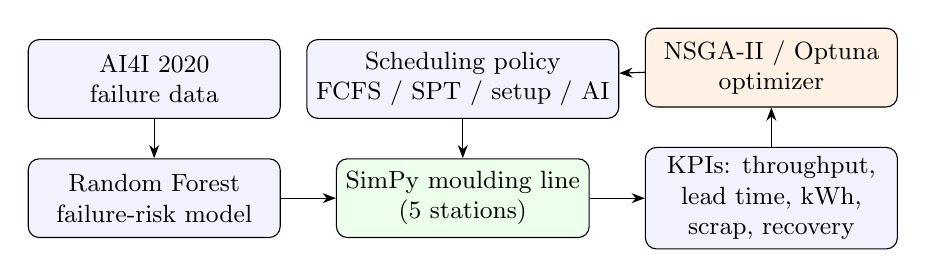
\begin{tikzpicture}[node distance=0.5cm and 0.7cm, every node/.style={font=\small}, box/.style={draw, rounded corners, align=center, minimum width=3.2cm, minimum height=1cm, fill=blue!5}]
\node[box] (data) {AI4I 2020\\failure data};
\node[box, below=of data] (ml) {Random Forest\\failure-risk model};
\node[box, right=of ml, fill=green!8] (sim) {SimPy moulding line\\(5 stations)};
\node[box, above=of sim] (pol) {Scheduling policy\\FCFS / SPT / setup / AI};
\node[box, right=of sim] (kpi) {KPIs: throughput,\\lead time, kWh,\\scrap, recovery};
\node[box, above=of kpi, fill=orange!10] (opt) {NSGA-II / Optuna\\optimizer};
\draw[-{Stealth}] (data) -- (ml);
\draw[-{Stealth}] (ml) -- (sim);
\draw[-{Stealth}] (pol) -- (sim);
\draw[-{Stealth}] (sim) -- (kpi);
\draw[-{Stealth}] (kpi) -- (opt);
\draw[-{Stealth}] (opt) -- (pol);
\end{tikzpicture}
\caption{Conceptual framework derived from the literature.}
\label{fig:concept}
\end{figure}

Three gaps emerge from the review.
\begin{enumerate}
  \item \textbf{Isolated objectives.} Scheduling studies with setups \cite{allahverdi2008} rarely model energy. Energy studies \cite{mouzon2007,gahm2016} rarely model breakdowns; Duan and Wang \cite{duan2021} add breakdowns but not setups or failure prediction. Rescheduling studies \cite{vieira2003,ouelhadj2009} rarely model energy or setups. Few studies treat changeovers, energy and disruptions together.
  \item \textbf{Missing peripheral loads.} Gahm et al.\ \cite{gahm2016} note that most energy-aware models ignore facility loads. Clean-room HVAC is a significant fixed load in medical moulding and is seldom modelled.
  \item \textbf{Limited reproducibility.} Reviews on machine learning in PPC and maintenance \cite{usuga2020,carvalho2019} report that private data and unpublished code limit reproducibility.
\end{enumerate}

Our project responds to all three gaps. It models changeovers, machine and clean-room energy, and failures in one simulation. It uses only public data and open-source tools. It reports results across many randomised scenarios shared by all policies, as Law \cite{law2015} recommends. We expect trade-offs rather than a single winning policy. For example, aggressive machine shutdown may save energy but extend lead time after a breakdown. The Pareto front will make such trade-offs visible to a production planner.

\subsection{Alignment with the Proposed Work}
Table~\ref{tab:align} links the insights from the literature to the design decisions of our project.

\begin{table}[h]
\centering
\small
\begin{tabularx}{\textwidth}{>{\raggedright}p{3cm}>{\raggedright}X>{\raggedright\arraybackslash}X}
\toprule
\textbf{Criteria} & \textbf{Research insight} & \textbf{Project decision} \\
\midrule
Baseline quality & Dispatching rules are transparent and robust \cite{pinedo2016,ouelhadj2009} & FCFS, SPT and a setup-aware rule as baselines \\
Changeovers & Ignoring setups yields infeasible schedules \cite{allahverdi2008} & Sequence-dependent mould changes plus GMP line clearance \\
Energy coverage & Idle energy and facility loads are significant \cite{mouzon2007,gahm2016} & Machine power states, idle shutdown and fixed HVAC load \\
Disruptions & Predictive plus reactive control is promising \cite{ouelhadj2009,duan2021} & Failure risk from a Random Forest feeds dispatching and maintenance decisions \\
Data availability & Private data limits reproducibility \cite{carvalho2019,matzka2020} & Public AI4I~2020 data and synthetic plant parameters \\
Valid comparison & Replications and common random numbers \cite{law2015} & Many randomised scenarios shared by all policies, confidence intervals \\
Conflicting goals & Pareto fronts expose trade-offs \cite{deb2002} & NSGA-II search via Optuna \cite{akiba2019} \\
\bottomrule
\end{tabularx}
\caption{Alignment of research insights with the proposed project design.}
\label{tab:align}
\end{table}

\section{Method Selection Justification}
\label{sec:justification}
The literature analysis led to the following choices for the project.

\subsection{Reasons for Selection}
\begin{itemize}
  \item \textbf{SimPy discrete-event simulation:} DES is the dominant method for testing control policies under uncertainty \cite{negahban2014}. SimPy is open source and process-based, which keeps the model reproducible \cite{simpy}.
  \item \textbf{FCFS, SPT and setup-aware baselines:} These rules are standard and transparent \cite{pinedo2016}. The setup-aware rule reflects the importance of sequence-dependent mould changes \cite{allahverdi2008}.
  \item \textbf{Random Forest on AI4I~2020:} Random Forest is the most frequently used predictive-maintenance method \cite{carvalho2019,breiman2001}. AI4I~2020 is public and labelled \cite{matzka2020}.
  \item \textbf{NSGA-II via Optuna:} NSGA-II returns a Pareto front instead of one weighted answer \cite{deb2002}. Optuna provides a maintained implementation with a simple Python interface \cite{akiba2019}.
  \item \textbf{Combined advantage:} Together these components cover changeovers, energy and disruptions in one simulation-optimization loop, which addresses the three gaps identified in Section~\ref{sec:synthesis}.
\end{itemize}

\section{Conclusion}
\label{sec:conclusion}
This bibliography report reviewed the literature behind our case study on a simulated medical injection-moulding line. The review began with Industry~4.0 and AI in production planning. It then narrowed to setup-aware scheduling, energy-efficient scheduling, dynamic rescheduling, predictive maintenance, discrete-event simulation and multi-objective optimization. It closed with the specific constraints of medical moulding at a site like Gerresheimer Pfreimd.

The review confirms that each method is well established on its own. Dispatching rules give transparent baselines. Machine turn-off policies reduce idle energy. Random Forests predict failures reliably on tabular data. NSGA-II produces Pareto fronts for conflicting objectives. Discrete-event simulation offers a safe and repeatable test environment. The main gap lies in combining these methods for a regulated, energy-intensive moulding process with open data and code.

The review has shaped several design decisions. We use FCFS, SPT and a setup-aware rule as baselines. We include clean-room HVAC as a fixed energy load. We train the failure model on AI4I~2020 and evaluate it with recall and F1-score. We compare policies on shared randomised scenarios with confidence intervals. The main limitation is that all factory parameters are synthetic. Our conclusions will therefore apply to simulated scenarios, and sensitivity analysis will test how robust they are. The next project phase will make the plant model more realistic, with more moulding machines and realistic lot sizes, and will repeat the tuning and held-out comparison.

\newpage
\begin{thebibliography}{99}
\addcontentsline{toc}{section}{References}

\bibitem{kagermann2013} H.~Kagermann, W.~Wahlster, and J.~Helbig, \emph{Recommendations for Implementing the Strategic Initiative INDUSTRIE 4.0: Final Report of the Industrie 4.0 Working Group}. Frankfurt am Main: acatech -- National Academy of Science and Engineering, 2013.

\bibitem{lee2015} J.~Lee, B.~Bagheri, and H.-A. Kao, ``A cyber-physical systems architecture for Industry 4.0-based manufacturing systems,'' \emph{Manufacturing Letters}, vol.~3, pp.~18--23, 2015. \href{https://doi.org/10.1016/j.mfglet.2014.12.001}{doi:10.1016/j.mfglet.2014.12.001}.

\bibitem{usuga2020} J.~P. Usuga Cadavid, S.~Lamouri, B.~Grabot, R.~Pellerin, and A.~Fortin, ``Machine learning applied in production planning and control: a state-of-the-art in the era of Industry 4.0,'' \emph{Journal of Intelligent Manufacturing}, vol.~31, no.~6, pp.~1531--1558, 2020. \href{https://doi.org/10.1007/s10845-019-01531-7}{doi:10.1007/s10845-019-01531-7}.

\bibitem{zhang2019} J.~Zhang, G.~Ding, Y.~Zou, S.~Qin, and J.~Fu, ``Review of job shop scheduling research and its new perspectives under Industry 4.0,'' \emph{Journal of Intelligent Manufacturing}, vol.~30, no.~4, pp.~1809--1830, 2019. \href{https://doi.org/10.1007/s10845-017-1350-2}{doi:10.1007/s10845-017-1350-2}.

\bibitem{pinedo2016} M.~L. Pinedo, \emph{Scheduling: Theory, Algorithms, and Systems}, 5th~ed. Cham: Springer, 2016. \href{https://doi.org/10.1007/978-3-319-26580-3}{doi:10.1007/978-3-319-26580-3}.

\bibitem{allahverdi2008} A.~Allahverdi, C.~T. Ng, T.~C.~E. Cheng, and M.~Y. Kovalyov, ``A survey of scheduling problems with setup times or costs,'' \emph{European Journal of Operational Research}, vol.~187, no.~3, pp.~985--1032, 2008. \href{https://doi.org/10.1016/j.ejor.2006.06.060}{doi:10.1016/j.ejor.2006.06.060}.

\bibitem{mouzon2007} G.~Mouzon, M.~B. Yildirim, and J.~Twomey, ``Operational methods for minimization of energy consumption of manufacturing equipment,'' \emph{International Journal of Production Research}, vol.~45, no.~18--19, pp.~4247--4271, 2007. \href{https://doi.org/10.1080/00207540701450013}{doi:10.1080/00207540701450013}.

\bibitem{gahm2016} C.~Gahm, F.~Denz, M.~Dirr, and A.~Tuma, ``Energy-efficient scheduling in manufacturing companies: A review and research framework,'' \emph{European Journal of Operational Research}, vol.~248, no.~3, pp.~744--757, 2016. \href{https://doi.org/10.1016/j.ejor.2015.07.017}{doi:10.1016/j.ejor.2015.07.017}.

\bibitem{vieira2003} G.~E. Vieira, J.~W. Herrmann, and E.~Lin, ``Rescheduling manufacturing systems: A framework of strategies, policies, and methods,'' \emph{Journal of Scheduling}, vol.~6, no.~1, pp.~39--62, 2003. \href{https://doi.org/10.1023/A:1022235519958}{doi:10.1023/A:1022235519958}.

\bibitem{duan2021} J.~Duan and J.~Wang, ``Energy-efficient scheduling for a flexible job shop with machine breakdowns considering machine idle time arrangement and machine speed level selection,'' \emph{Computers \& Industrial Engineering}, vol.~161, art.~107677, 2021. \href{https://doi.org/10.1016/j.cie.2021.107677}{doi:10.1016/j.cie.2021.107677}.

\bibitem{ouelhadj2009} D.~Ouelhadj and S.~Petrovic, ``A survey of dynamic scheduling in manufacturing systems,'' \emph{Journal of Scheduling}, vol.~12, no.~4, pp.~417--431, 2009. \href{https://doi.org/10.1007/s10951-008-0090-8}{doi:10.1007/s10951-008-0090-8}.

\bibitem{carvalho2019} T.~P. Carvalho, F.~A. A. M.~N. Soares, R.~Vita, R.~da~P. Francisco, J.~P. Basto, and S.~G.~S. Alcal\'a, ``A systematic literature review of machine learning methods applied to predictive maintenance,'' \emph{Computers \& Industrial Engineering}, vol.~137, art.~106024, 2019. \href{https://doi.org/10.1016/j.cie.2019.106024}{doi:10.1016/j.cie.2019.106024}.

\bibitem{matzka2020} S.~Matzka, ``Explainable artificial intelligence for predictive maintenance applications,'' in \emph{Proc. 3rd Int. Conf. on Artificial Intelligence for Industries (AI4I)}, 2020, pp.~69--74. \href{https://doi.org/10.1109/AI4I49448.2020.00023}{doi:10.1109/AI4I49448.2020.00023}.

\bibitem{breiman2001} L.~Breiman, ``Random forests,'' \emph{Machine Learning}, vol.~45, no.~1, pp.~5--32, 2001. \href{https://doi.org/10.1023/A:1010933404324}{doi:10.1023/A:1010933404324}.

\bibitem{pedregosa2011} F.~Pedregosa \emph{et al.}, ``Scikit-learn: Machine learning in Python,'' \emph{Journal of Machine Learning Research}, vol.~12, pp.~2825--2830, 2011.

\bibitem{law2015} A.~M. Law, \emph{Simulation Modeling and Analysis}, 5th~ed. New York: McGraw-Hill Education, 2015.

\bibitem{negahban2014} A.~Negahban and J.~S. Smith, ``Simulation for manufacturing system design and operation: Literature review and analysis,'' \emph{Journal of Manufacturing Systems}, vol.~33, no.~2, pp.~241--261, 2014. \href{https://doi.org/10.1016/j.jmsy.2013.12.007}{doi:10.1016/j.jmsy.2013.12.007}.

\bibitem{simpy} SimPy Developers, ``SimPy: Discrete event simulation for Python,'' Documentation. [Online]. Available: \url{https://simpy.readthedocs.io}

\bibitem{deb2002} K.~Deb, A.~Pratap, S.~Agarwal, and T.~Meyarivan, ``A fast and elitist multiobjective genetic algorithm: NSGA-II,'' \emph{IEEE Transactions on Evolutionary Computation}, vol.~6, no.~2, pp.~182--197, 2002. \href{https://doi.org/10.1109/4235.996017}{doi:10.1109/4235.996017}.

\bibitem{akiba2019} T.~Akiba, S.~Sano, T.~Yanase, T.~Ohta, and M.~Koyama, ``Optuna: A next-generation hyperparameter optimization framework,'' in \emph{Proc. 25th ACM SIGKDD Int. Conf. on Knowledge Discovery \& Data Mining}, 2019, pp.~2623--2631. \href{https://doi.org/10.1145/3292500.3330701}{doi:10.1145/3292500.3330701}.

\bibitem{rosato2000} D.~V. Rosato, D.~V. Rosato, and M.~G. Rosato, \emph{Injection Molding Handbook}, 3rd~ed. Boston: Kluwer Academic Publishers, 2000.

\bibitem{thiriez2006} A.~Thiriez and T.~Gutowski, ``An environmental analysis of injection molding,'' in \emph{Proc. IEEE Int. Symp. on Electronics and the Environment}, 2006, pp.~195--200. \href{https://doi.org/10.1109/ISEE.2006.1650060}{doi:10.1109/ISEE.2006.1650060}.

\bibitem{eugmp2022} European Commission, \emph{EudraLex Volume 4 -- EU Guidelines for Good Manufacturing Practice, Annex 1: Manufacture of Sterile Medicinal Products}. Brussels, 2022.

\bibitem{iso50001} International Organization for Standardization, \emph{ISO 50001:2018 -- Energy management systems: Requirements with guidance for use}. Geneva: ISO, 2018.

\bibitem{gx_pfreimd} Gerresheimer AG, ``Pfreimd, Germany -- Gerresheimer Regensburg GmbH,'' company location page. [Online]. Available: \url{https://www.gerresheimer.com/en/company/locations/pfreimd-germany}. Accessed: 31 Oct. 2026.

\end{thebibliography}

\end{document}
